	\begin{figure}[!h]
		\centering
 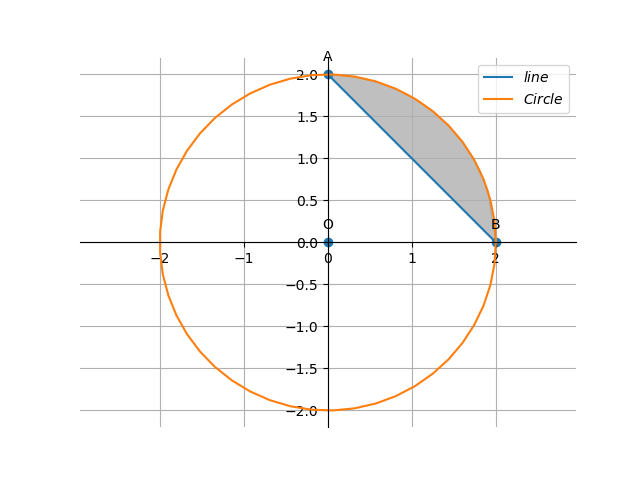
\includegraphics[width=\columnwidth]{chapters/12/8/2/6/figs/conic.png}
		\caption{}
		\label{fig:12/8/2/6}
  	\end{figure}
The given circle can be expressed as conics with parameters,
\begin{align}
\vec{V}=\myvec{
4 & 0\\
0 & 4
},
\vec{u}=0,
f=-16
\end{align}
The line parameters are
\begin{align}
\vec{h} &= \myvec{
2\\
0
}, 
\vec{m} = \myvec{\frac{1}{2} \\ -\frac{1}{2}}
\end{align}
Substituting the parameters in \eqref{eq:tangent_roots},
\begin{align}
\kappa =0,-4
\end{align}
yielding the points of intersection as
\begin{align}
    \vec{A}=\myvec{
0\\
2
    },
    \vec{B}=\myvec{
2\\
0
    }
\end{align}
From 
		\figref{fig:12/8/2/6},
the desired area is
\begin{align}
\int_{0}^{2}\sqrt{4-x^2} \,dx 
-\int_{0}^{2} (2-x) \,dx
=\pi - 2
\end{align}
